\chapter{Results and Discussion}

\section{Running procedure}
\label{sec:prog}
The \machine features a classical software interface which takes text files containing the information of a Hamiltonian like Table \ref{tab:eg_sat_full}.  After this is uploaded the machine anneals the Hamiltonian as described in Chapter \ref{chap:machine} and returns the values of the spins it found after annealing.

Each time the machine loads a Hamiltonian it programs in the fields and couplings as described in Section \ref{sec:machine_prog}, it can evaluate the Hamiltonian many times.  Each time the\machine loads in a Hamiltonian we call a \emph{run}, while each repetition of the same Hamiltonian without loading we call a \emph{read}.  Any programming error (see \ref{sec:noise}) in the Hamiltonian should be the same between reads and differ between runs.

The state read out after each read is either the ground state, or some other higher energy (and incorrect) state.  The successes and failures thus follow a binomial distribution; there is some probability $p$ of getting the ground state, and probability $1-p$ of getting a different state.
Our best estimate of the fidelity from a single run is thus the fraction of successes, or $p = \frac{gs}{n}$ for $gs$ reads of the ground state and $n$ total reads.  We can also estimate the error in our estimate of the fidelity, because the variance of a binomial distribution is $\sigma^2 = np(1-p)$.

\section{Single Qubyte Hamiltonian}
The first Hamiltonian evaluated was very similar to the Hamiltonian described in Table \ref{tab:eg_sat_full} to encode a single clause SAT problem.  The Hamiltonian ``k44'' is shown in table \ref{tab:k44}, consisting of a single qubyte of spins and encoding the logic of a single SAT clause was evaluated in with runs at anneal times from 20 $\mu$s to 500 $\mu$s with 1000 reads per run.  One thousand repetitions at a given anneal time will give us good statistics to estimate the fidelity.

Figure \ref{fig:k44_comparison} shows the results of two such sweeps.  The fidelity was estimated as described in Section \ref{sec:prog}.  First, contrary to our expectations, the fidelity \emph{decreases} as the anneal time increases.  We would expect that longer anneal times bring us closer to adiabatic evolution and thus remaining in the ground state.  This result suggests to us that adiabaticity (or lack thereof) is not dominating the fidelity for long annealing times. 
Second, there is significant change in the fidelity over very small changes in anneal time for less than $\sim 300$ $\mu$s, well outside what we would statistically expect based on the number of reads conducted if the cause is simple statistical noise.  This suggests that there is something going on besides the annealing time that determines the fidelity when the anneal time is short.  This factor disappears for longer anneal times, when whatever is damping the fidelity also seems to dampen the short time oscillations.
\begin{table}
	\begin{center}
\begin{tabular}{ | l | l | l | l |}
	\hline
	\multicolumn{4}{|c|}{k44 Hamiltonian} \\ \hline
	\multicolumn{2}{|c|}{Fields} & \multicolumn{2}{c|}{Couplings} \\ \hline
	A & 1.0 & A,B & 1.0 \\
	B & 1.0 & A,D & -2.0 \\
	C & -1.0 & B,D & -2.0 \\
	D & -3.0 & C,D & 1.0 \\ \hline
\end{tabular}
\end{center}
\caption[k44 Hamiltonian]{The fields and couplings making up the Hamiltonian ``k44''.}
\label{tab:k44}
\end{table}

\begin{figure}
	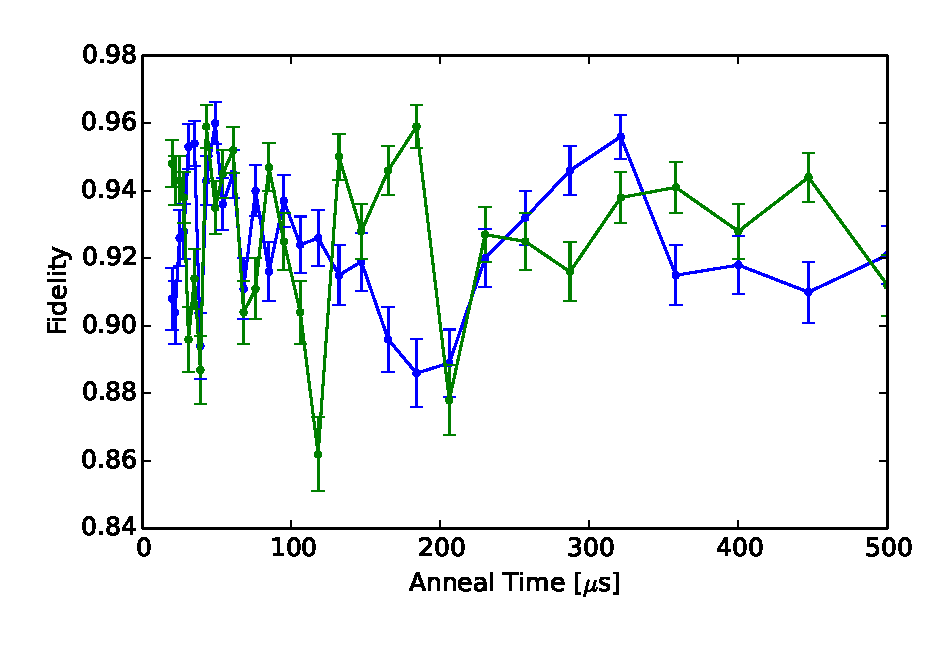
\includegraphics{img/k44.eps}
	\caption[Single K44 Fidelity]{Fidelity as a function of anneal time for the Hamiltonian ``k44'' which consists of a single SAT clause embedded into a single qubyte.  The error bars are estimated from the standard deviation of a binomial distribution of the reads.}
	\label{fig:k44_comparison}
\end{figure}


\section{Non-degenerate Single Qubyte Hamiltonian}

\begin{table}
	\begin{center}
\begin{tabular}{ | l | l | l | l |}
	\hline
	\multicolumn{4}{|c|}{k44\_and Hamiltonian} \\ \hline
	\multicolumn{2}{|c|}{Fields} & \multicolumn{2}{c|}{Couplings} \\ \hline
	A & 1.0 & A,B & 1.0 \\
	B & -1.0 & A,D & -2.0 \\
	C & 3.0 & B,D & -2.0 \\
	D & -1.0 & C,D & -1.0 \\ \hline
\end{tabular}
\end{center}
\caption[k44\_and Hamiltonian]{The fields and couplings that make up the Hamiltonian ``k44\_and''.  This single qubyte Hamiltonian has a single non-degenerate ground state: $\ket{\uparrow\uparrow\downarrow\uparrow}$ }
\label{tab:k44_and}
\end{table}
It was thought initially that the reason for the variability of the fidelity at short anneal times was due to the degeneracy of the ``k44'' Hamiltonian ground states.  The Hamiltonian ``k44\_and'' was created to be similar in form (same number of qubits) but having only a single ground state.  This Hamiltonian was evaluated for times ranging from 20 $\mu$s to 20 ms, with 4 runs taken at each time point and 100 reads per run.  Figure \ref{fig:results_avg} shows these results.  Each run produced as estimated fidelity as in Section \ref{sec:prog}, and the results shown here were synthesized by making a weighted average of each of the individual run's estimated fidelities.  The error bars shown here are the standard deviations of the means of the weighted averages, so small when the four runs produced nearly the same result and large when there was a large spread.  The short time oscillations are not entirely removed, although our estimates of the standard deviation matches up to the observed data much better; the trend of the data points falls almost entirely within the error bars.

\begin{figure}
	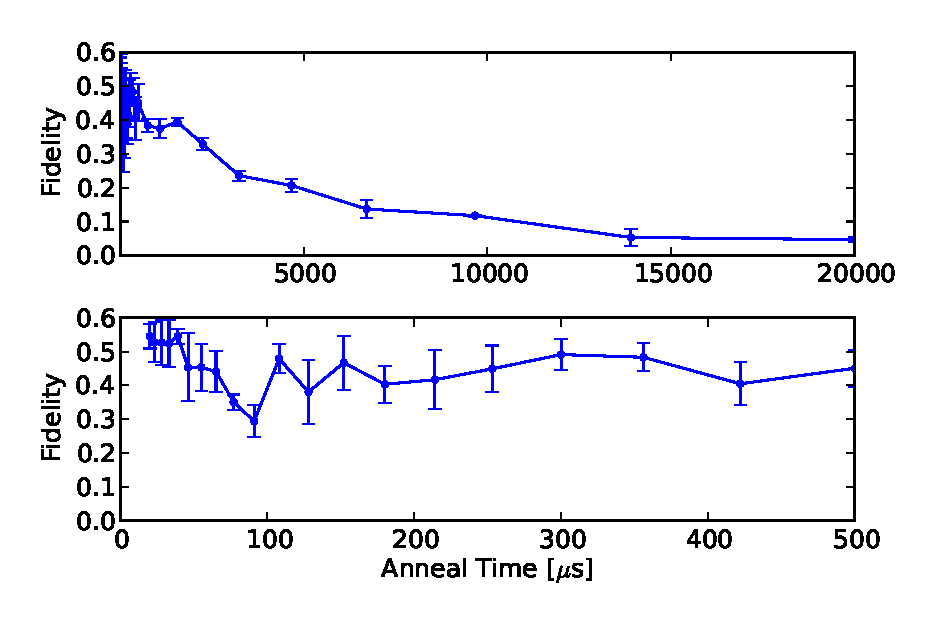
\includegraphics{img/final_single_k44.eps}
	\caption[Averaged Anneal Results]{Fidelity vs anneal time with each data point averaged over four different runs for the single qubyte ``k44\_and'' with a clone coupling value of -9.  Each run was used to estimate the fidelity independently, with the final estimate the weighted average of each run.  The errorbars reflect the standard deviation of the distribution of estimates of the runs.}
	\label{fig:results_avg}
\end{figure}




\section{Clone coupling value}
\label{sec:coupling}

\begin{figure}
	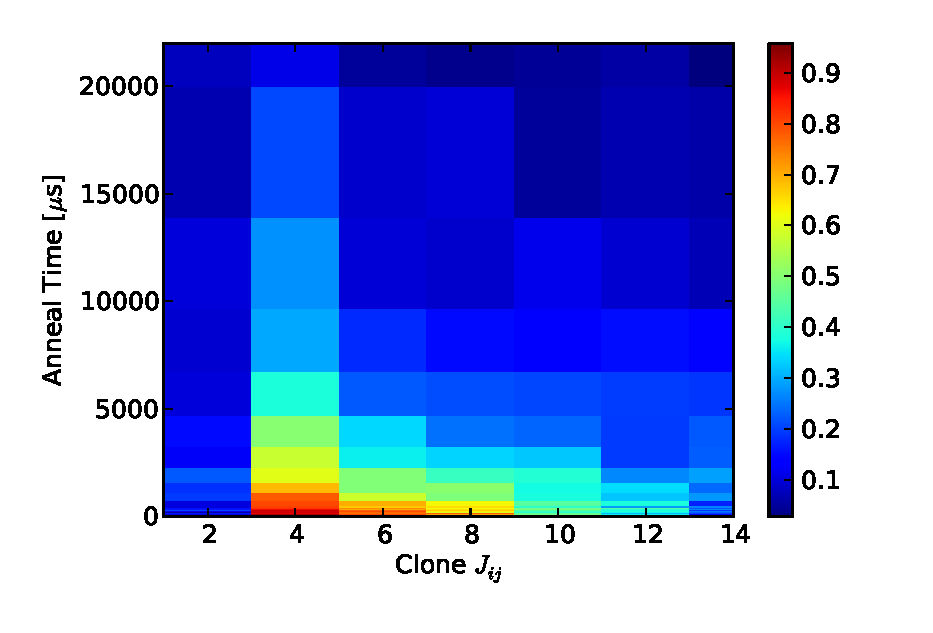
\includegraphics{img/n_8_t_v_c.eps}
	\caption[Variable Clone Coupling Fidelity]{Heat map of the fidelity as a function of anneal time and clone coupling value for the single qubyte ``k44\_and''.  The measured fidelity drops of rapidly with increasing clone coupling, but low clone coupling values do not preserve the ground state intact.  The sudden drop in fidelity at the smallest clone coupling value is caused by incorrect states with the same energy as the ground state.}
	\label{fig:clone_coupling}
\end{figure}

As discussed in Sections \ref{sec:embed_algo} and \ref{sec:resolution}, while for an ideal machine maximizing the clone coupling value would ensure that adding clones did not alter the ground states of our problem Hamiltonians, the \machine machine can only implement 15 different clone coupling values.  In addition, these values must be evenly spaced.  If we were to use a clone coupling value of $-14$ in a problem Hamiltonian which natively had coupling values of $-2,-1,1,2$, this would result in compressing each of the positive and negative couplings into one machine value.  The machine only implements couplings of the form 
\begin{equation}
	\pm\frac{x}{7}, 1 \le x \le 7
\end{equation}
so the above example would result in a physically implemented Hamiltonian of -1/7, -1/7, 1/7, $1/7$ in addition to the clone coupling of $-1$.  Most of the time this will result in a malformed Hamiltonian with incorrect ground states.

In addition to incorrect ground states, it is possible that the programming error in the machine is large enough to make the couplings $1/7$ and $2/7$ close enough to be likely to collide, whereas $1/7$ and $3/7$ could be far enough apart to be programmed correctly every time.  This could mean that even in scenarios where \machine has enough range to encode the problem Hamiltonian couplings correctly with a large clone coupling value we still don't want to do so.

This means that when selecting a clone coupling value we must balance these two competing factors, the desire to make the clone coupling as large as possible from a Hamiltonian correctness standpoint, and the desire to make it as small as possible from a machine resolution viewpoint.  The Hamiltonian correctness issue is correctness and knowable at the time the Hamiltonian is constructed; however in general to know whether a given clone coupling is large enough or not requires diagonalizing the Hamiltonian, and if this were possible then that would enable us to solve the initial computational problem directly.
The machine resolution problem is not necessarily the same from run to run; it could be that the compression of the problem Hamiltonian caused by the clone coupling value only makes it more likely for the machine to end up in an excited state.

\begin{figure}
	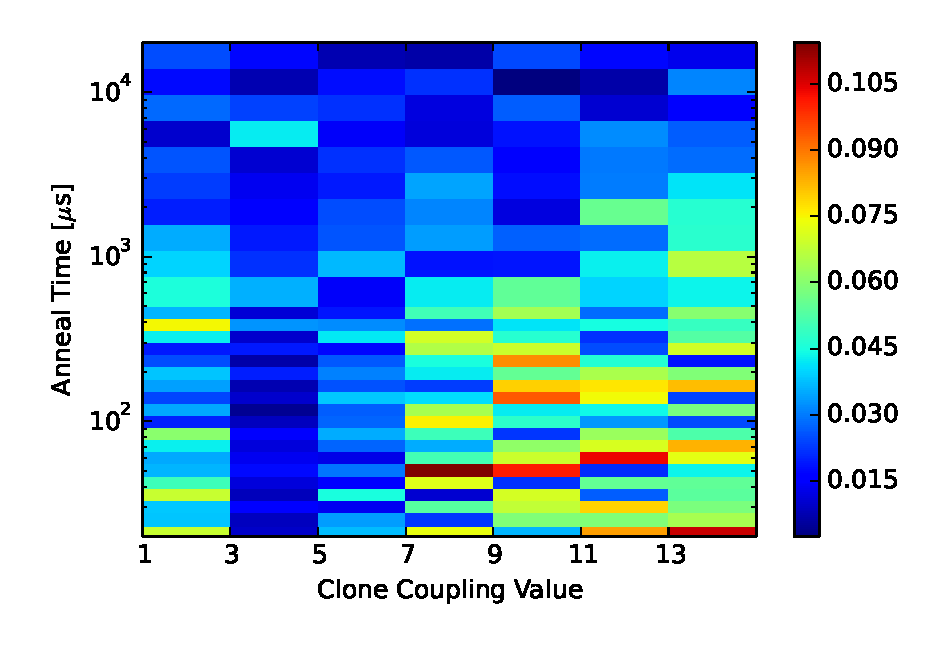
\includegraphics{img/t_c.eps}
	\caption[Fidelity Standard Deviation]{Heat map of the standard deviation of the estimated fidelity as a function of clone coupling value and annealing time for the single qubyte ``k44\_and''.  After $\sim$ 1000 $\mu$s the error drops down as we enter the long-time regime and the short-time oscillations die off.  The spread of the fidelity is also much lower for a clone coupling value of -3, which corresponds to the higher fidelities.}
	\label{fig:std_time}
\end{figure}

To empirically examine the impact of the value of the clone coupling, the ``k44\_and'' Hamiltonian was embedded multiple different times with a clone coupling value ranging from -1 to -14 (from the smallest coupling in the problem Hamiltonian to twice the native resolution of the machine).  Figure \ref{fig:clone_coupling} shows a heat map of the results of annealing these Hamiltonians from 20 $\mu$s to 20 ms.  Not only does fidelity increase as the clone coupling value is decreased, the short-time oscillations that we saw in the earlier results of ``k44'' in Figure \ref{fig:k44_comparison} are removed.  This is shown very clearly in Figure \ref{fig:std_time}, which displays the standard deviation of the estimated fidelity as a function of anneal time and clone coupling value.

At longer anneal times the difference in fidelity is reduced, and the same long-time drop in fidelities that was observed in other Hamiltonians continues.  This means that the mechanism for the long-time fidelity drop is not strongly impacted by the clone coupling value.

The fidelity drops off strongly from its peak at a clone coupling value of -3.  Each of the higher clone coupling values corresponds to more and more compression of the computational couplings into fewer physical couplings.  This pattern does not continue to the -1 coupling, because that clone coupling value results in a malformed Hamiltonian where a domain wall forms in the ferromagnetic couplings, leading to what should be an excited state having the same energy as the ground state.  The ``k44\_and'' Hamiltonian's largest coupling value is $|3.0|$, which suggests that a clone coupling value of -3 performs well because it does not compress any couplings together.

\section{Size scaling}
The size scaling behaviour of ``k44\_and'' was also studied.  This was done by copy and pasting the fields and couplings over to new qubytes.  The resulting Hamiltonian still encodes the same SAT problem as the original ``k44\_and'', and still only has one ground state, but is able to be scaled from 1 to 55 qubytes, a range of 8 to 440 spins.  Figure \ref{fig:time_spins} shows the fidelity plotted against anneal time and number of spins, for the clone coupling value which maximizes fidelity (-3).  The same plot for other clone couplings looks similar but with lower fidelity values across the board.  Larger Hamiltonians show similar behaviour to the original one qubyte ``k44\_and'', but fall off even faster with increased anneal time.

\begin{figure}
	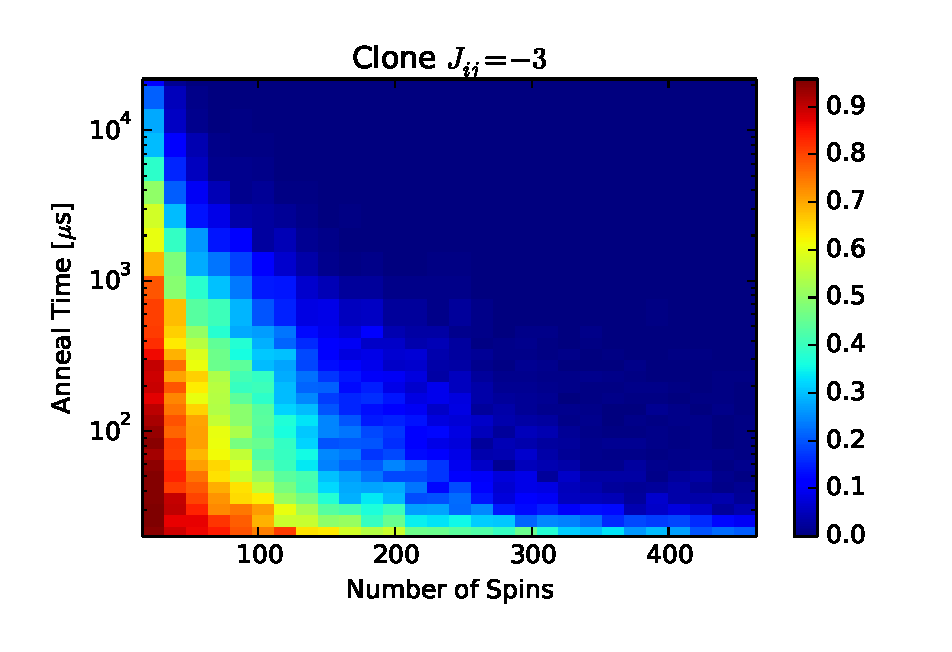
\includegraphics{img/pcolor_c_3.eps}
	\caption[Fidelity vs Time vs Number of Qubits]{Heat map of the estimated fidelity as a function of annealing time and number of spins in the Hamiltonian, with a clone coupling value of -3.}
	\label{fig:time_spins}
\end{figure}

\begin{figure}
	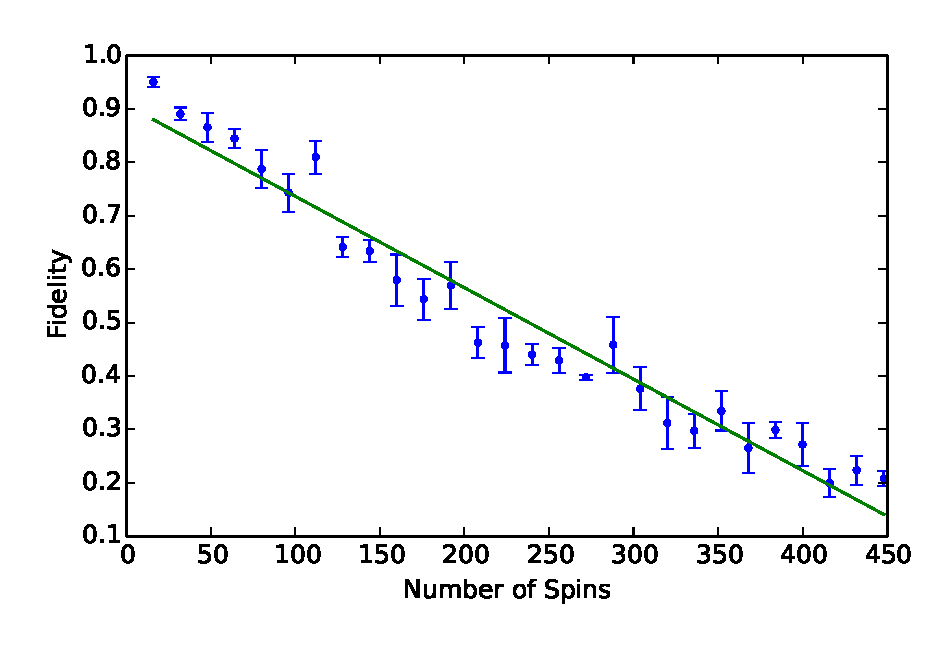
\includegraphics{img/trend.eps}
	\caption[Fidelity vs Number of Qubits]{Fidelity as a function of number of qubits for an anneal time of 20 $\mu$s and a clone coupling value of -3 as well as line of best fit.}
	\label{fig:trend}
\end{figure}

Figure \ref{fig:trend} shows the fidelity for annealing for 20 $\mu$s with a clone coupling value of -3 (that is, the values which maximize fidelity) as a function of number of spins.  The result is very close to a straight line; a linear regression is shown against the data.  This result would seem to indicate that for this particular set of parameters (anneal time of 20 $\mu$s, clone coupling value of -3) the \machine machine scales linearly.  This is what we would expect if there was a some success probability for a given single ``k44\_and'' unit cell, where the total success probability being the product of each one succeeding individually.

\section{Boolean SAT Hamiltonian}
The last investigation was conducted on a six variable, 21 clause 3-SAT Hamiltonian with two satisfying assignments, \texttt{(ttftft,ttttft)}.  When embedded this Hamiltonian filled essentially the entire hardware graph.  Figure \ref{fig:test_6} shows the estimated fidelity from anneal times ranging from 20 $\mu$s to 500 $\mu$s, estimated from 1000 reads and single runs at each anneal time.  The fidelity is close to zero throughout the time range.  In contrast to our previously observed Hamiltonians, the \machine machine seems unable to successfully solve this particular problem instance.

Figure \ref{fig:test_6_hist} is a pair of histograms showing all 1000 results of annealing at 20 $\mu$s for both the ``6\_018'' Hamiltonian and the 3-SAT Hamiltonian.  The peak of the distribution for ``6\_018'' is near the ground state, while the peak of the distribution for the 3-SAT Hamiltonian is in the neighbourhood of the 10th excited state.  Presumably this is due to the energy levels of the 3-SAT Hamiltonian closing together where the ``6\_018'' levels do not.  The distribution of the results for the 3-SAT Hamiltonian is also broader, for reasons which are not clear.  Both of these Hamiltonians are much to large to be simulated classically, so we cannot predict how the energy levels change over the annealing to explain the distribution differences directly.

\begin{figure}
	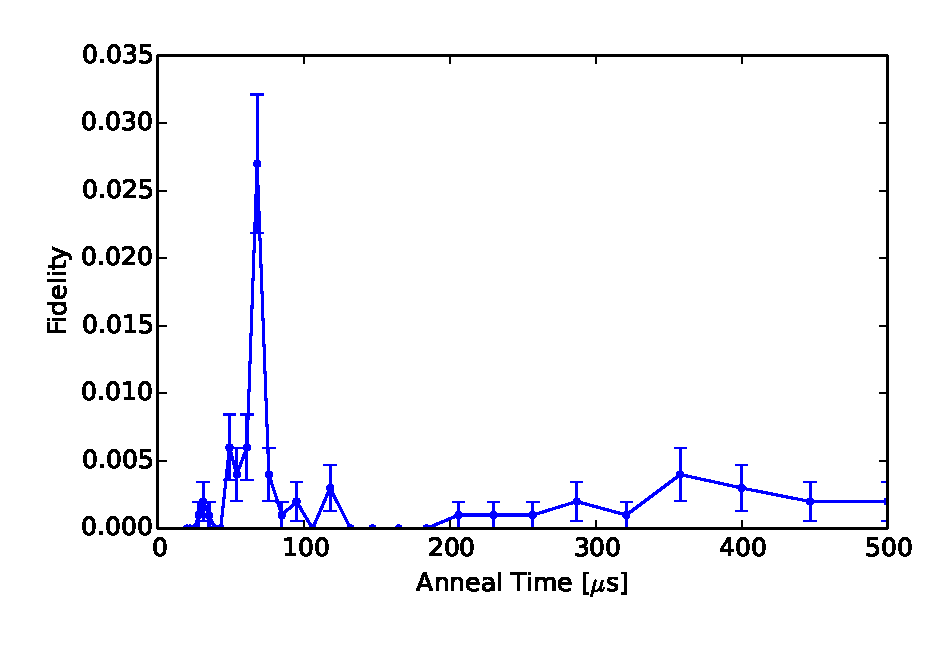
\includegraphics{img/test_6.eps}
	\caption[Result of a 6 Variable 3-SAT Instance]{This figure shows the estimated fidelity as a function of annealing time for a six variable, 21 clause 3-SAT instance.  The fidelity is essentially zero throughout the time range.}
	\label{fig:test_6}
\end{figure}

\begin{figure}
	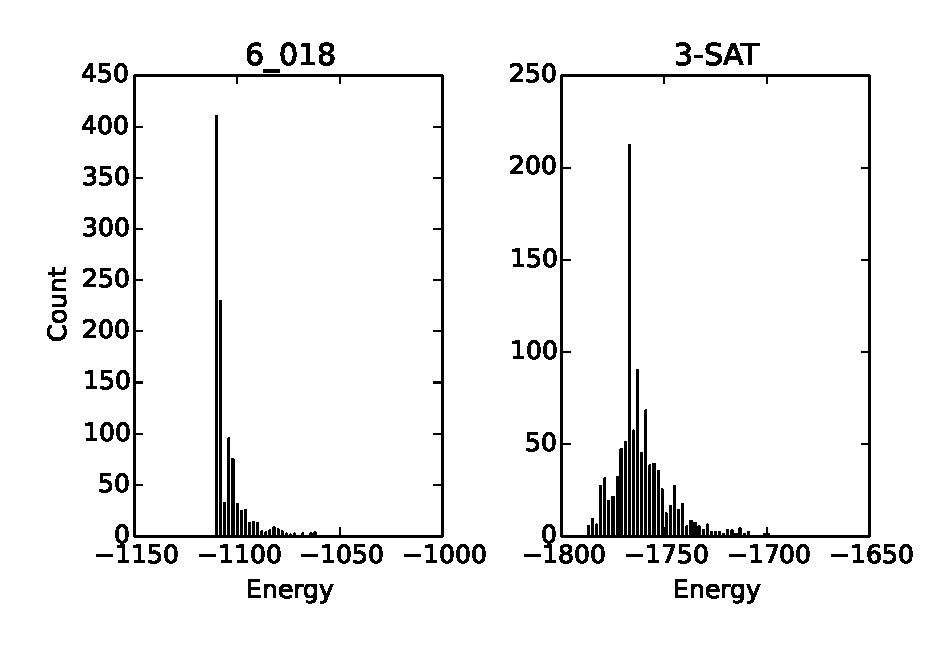
\includegraphics{img/hist.eps}
	\caption[20 $\mu$s Result State Histograms]{Histograms showing all 1000 states found after 20 $\mu$s of annealing for both ``6\_018'' on the left and the 6 variable 3-SAT on the right.  The fidelity is clearly much higher on the left.  While the distribution of the ``6\_018'' results peaks near the ground state and decays exponentially, the 3-SAT results are peaked in the vicinity of the 10th excited state.}
	\label{fig:test_6_hist}
\end{figure}

